\begin{figure}[H]
    \centering
    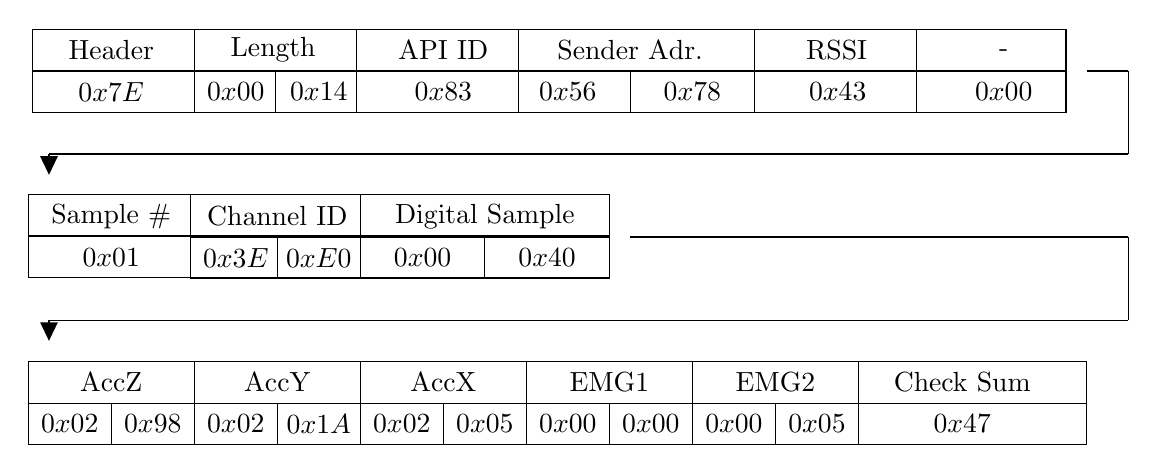
\begin{tikzpicture}[x=0.75pt,y=0.75pt,yscale=-1,xscale=1]
%uncomment if require: \path (0,230.14285278320312); %set diagram left start at 0, and has height of 230.14285278320312

%Shape: Rectangle [id:dp10856467985503815] 
\draw   (22,10) -- (520,10) -- (520,50) -- (22,50) -- cycle ;
%Shape: Rectangle [id:dp1921303622580388] 
\draw   (22,10) -- (100,10) -- (100,30) -- (22,30) -- cycle ;
%Shape: Rectangle [id:dp5511536446299157] 
\draw   (22,30) -- (100,30) -- (100,50) -- (22,50) -- cycle ;
%Shape: Rectangle [id:dp8551124842169571] 
\draw   (100,30) -- (178,30) -- (178,50) -- (100,50) -- cycle ;
%Shape: Rectangle [id:dp1542301721460031] 
\draw   (100,10) -- (178,10) -- (178,30) -- (100,30) -- cycle ;
%Shape: Rectangle [id:dp39637490877675896] 
\draw   (100,30) -- (139,30) -- (139,50) -- (100,50) -- cycle ;
%Shape: Rectangle [id:dp7008641367286479] 
\draw   (178,10) -- (256,10) -- (256,30) -- (178,30) -- cycle ;
%Shape: Rectangle [id:dp6311822380704302] 
\draw   (178,30) -- (256,30) -- (256,50) -- (178,50) -- cycle ;
%Shape: Rectangle [id:dp2794130706147937] 
\draw   (256,10) -- (370,10) -- (370,30) -- (256,30) -- cycle ;
%Shape: Rectangle [id:dp0748834298647747] 
\draw   (256,30) -- (370,30) -- (370,50) -- (256,50) -- cycle ;
%Shape: Rectangle [id:dp3442757233060003] 
\draw   (256,30) -- (310,30) -- (310,50) -- (256,50) -- cycle ;
%Shape: Rectangle [id:dp7243088972581471] 
\draw   (370,10) -- (448,10) -- (448,30) -- (370,30) -- cycle ;
%Shape: Rectangle [id:dp8634226198686377] 
\draw   (370,30) -- (448,30) -- (448,50) -- (370,50) -- cycle ;
%Shape: Rectangle [id:dp049451176775102246] 
\draw   (448,30) -- (520,30) -- (520,50) -- (448,50) -- cycle ;
%Shape: Rectangle [id:dp10185955763756471] 
\draw   (448,10) -- (520,10) -- (520,30) -- (448,30) -- cycle ;
%Shape: Rectangle [id:dp3116685664620873] 
\draw   (20,89.5) -- (300,89.5) -- (300,129.5) -- (20,129.5) -- cycle ;
%Shape: Rectangle [id:dp4024383934360989] 
\draw   (20,89.5) -- (98,89.5) -- (98,109.5) -- (20,109.5) -- cycle ;
%Shape: Rectangle [id:dp9664793454969085] 
\draw   (20,109.5) -- (98,109.5) -- (98,129.5) -- (20,129.5) -- cycle ;
%Shape: Rectangle [id:dp4124508293977984] 
\draw   (98,109.5) -- (180,109.5) -- (180,129.5) -- (98,129.5) -- cycle ;
%Shape: Rectangle [id:dp711781414287457] 
\draw   (98,89.5) -- (180,89.5) -- (180,110) -- (98,110) -- cycle ;
%Shape: Rectangle [id:dp356328253424953] 
\draw   (98,110) -- (140,110) -- (140,130) -- (98,130) -- cycle ;
%Shape: Rectangle [id:dp6733077815498894] 
\draw   (180,89.5) -- (300,89.5) -- (300,110) -- (180,110) -- cycle ;
%Shape: Rectangle [id:dp6479637887159722] 
\draw   (180,109.5) -- (300,109.5) -- (300,130) -- (180,130) -- cycle ;
%Shape: Rectangle [id:dp19346515996870206] 
\draw   (180,110) -- (240,110) -- (240,130) -- (180,130) -- cycle ;
%Shape: Rectangle [id:dp38146177317207886] 
\draw   (20,170) -- (530,170) -- (530,210) -- (20,210) -- cycle ;
%Shape: Rectangle [id:dp4556101293933754] 
\draw   (20,170) -- (100,170) -- (100,190) -- (20,190) -- cycle ;
%Shape: Rectangle [id:dp5407175554825892] 
\draw   (20,190) -- (60,190) -- (60,210) -- (20,210) -- cycle ;
%Shape: Rectangle [id:dp7450461679704352] 
\draw   (60,190) -- (100,190) -- (100,210) -- (60,210) -- cycle ;
%Shape: Rectangle [id:dp4332754864269053] 
\draw   (100,170) -- (180,170) -- (180,190) -- (100,190) -- cycle ;
%Shape: Rectangle [id:dp28452698286293754] 
\draw   (140,190) -- (180,190) -- (180,210) -- (140,210) -- cycle ;
%Shape: Rectangle [id:dp7914115317030024] 
\draw   (100,190) -- (140,190) -- (140,210) -- (100,210) -- cycle ;
%Shape: Rectangle [id:dp38727788354631554] 
\draw   (220,190) -- (260,190) -- (260,210) -- (220,210) -- cycle ;
%Shape: Rectangle [id:dp22288528455712386] 
\draw   (180,190) -- (220,190) -- (220,210) -- (180,210) -- cycle ;
%Shape: Rectangle [id:dp8165391393896375] 
\draw   (180,170) -- (260,170) -- (260,190) -- (180,190) -- cycle ;
%Shape: Rectangle [id:dp6523955550843537] 
\draw   (260,190) -- (300,190) -- (300,210) -- (260,210) -- cycle ;
%Shape: Rectangle [id:dp9747757771531758] 
\draw   (300,190) -- (340,190) -- (340,210) -- (300,210) -- cycle ;
%Shape: Rectangle [id:dp8745951425419776] 
\draw   (260,170) -- (340,170) -- (340,190) -- (260,190) -- cycle ;
%Shape: Rectangle [id:dp9793885365492223] 
\draw   (340,170) -- (420,170) -- (420,190) -- (340,190) -- cycle ;
%Shape: Rectangle [id:dp03157812028724449] 
\draw   (340,190) -- (380,190) -- (380,210) -- (340,210) -- cycle ;
%Shape: Rectangle [id:dp24057366681022452] 
\draw   (380,190) -- (420,190) -- (420,210) -- (380,210) -- cycle ;
%Shape: Rectangle [id:dp36093082441092617] 
\draw   (140,110) -- (180,110) -- (180,130) -- (140,130) -- cycle ;
%Shape: Rectangle [id:dp7171363093153074] 
\draw   (420,170) -- (530,170) -- (530,190) -- (420,190) -- cycle ;
%Shape: Rectangle [id:dp5647098232631986] 
\draw   (420,190) -- (530,190) -- (530,210) -- (420,210) -- cycle ;
%Straight Lines [id:da6332689457085323] 
\draw    (530,30) -- (550,30) ;


%Straight Lines [id:da30561509563968503] 
\draw    (550,30) -- (550,70) ;


%Straight Lines [id:da09566559311573841] 
\draw    (550,70) -- (30,70) ;


%Straight Lines [id:da5601518731242143] 
\draw    (30,70) -- (30,78) ;
\draw [shift={(30,80)}, rotate = 270] [fill={rgb, 255:red, 0; green, 0; blue, 0 }  ][line width=0.75]  [draw opacity=0] (8.93,-4.29) -- (0,0) -- (8.93,4.29) -- cycle    ;

%Straight Lines [id:da9169109459317539] 
\draw    (310,110) -- (550,110) ;


%Straight Lines [id:da5912944234587121] 
\draw    (550,110) -- (550,150) ;


%Straight Lines [id:da7375405804531086] 
\draw    (550,150) -- (30,150) ;


%Straight Lines [id:da024754719673693026] 
\draw    (30,150) -- (30,158) ;
\draw [shift={(30,160)}, rotate = 270] [fill={rgb, 255:red, 0; green, 0; blue, 0 }  ][line width=0.75]  [draw opacity=0] (8.93,-4.29) -- (0,0) -- (8.93,4.29) -- cycle    ;


% Text Node
\draw (60,20) node  [align=left] {Header};
% Text Node
\draw (60,40) node   {$0x7E$};
% Text Node
\draw (138,19.5) node  [align=left] {Length};
% Text Node
\draw (120,40) node   {$0x00$};
% Text Node
\draw (160,40) node   {$0x14$};
% Text Node
\draw (220,20) node  [align=left] {API ID};
% Text Node
\draw (220,40) node   {$0x83$};
% Text Node
\draw (310,20) node  [align=left] {Sender Adr.};
% Text Node
\draw (280,40) node   {$0x56$};
% Text Node
\draw (340,40) node   {$0x78$};
% Text Node
\draw (409.5,20) node  [align=left] {RSSI};
% Text Node
\draw (410,40) node   {$0x43$};
% Text Node
\draw (490,20) node  [align=left] {\mbox{-}};
% Text Node
\draw (490,40) node   {$0x00$};
% Text Node
\draw (60,100) node  [align=left] {Sample \#};
% Text Node
\draw (60,120) node   {$0x01$};
% Text Node
\draw (140,100) node  [align=left] {Channel ID};
% Text Node
\draw (120,120) node   {$0x3E$};
% Text Node
\draw (160,120) node   {$0xE0$};
% Text Node
\draw (240,100) node  [align=left] {Digital Sample};
% Text Node
\draw (210,120) node   {$0x00$};
% Text Node
\draw (270,120) node   {$0x40$};
% Text Node
\draw (60,180) node  [align=left] {AccZ};
% Text Node
\draw (40,200) node   {$0x02$};
% Text Node
\draw (80,200) node   {$0x98$};
% Text Node
\draw (140,180) node  [align=left] {AccY};
% Text Node
\draw (120,200) node   {$0x02$};
% Text Node
\draw (160,200) node   {$0x1A$};
% Text Node
\draw (220,180) node  [align=left] {AccX};
% Text Node
\draw (200,200) node   {$0x02$};
% Text Node
\draw (240,200) node   {$0x05$};
% Text Node
\draw (280,200) node   {$0x00$};
% Text Node
\draw (320,200) node   {$0x00$};
% Text Node
\draw (300,180) node  [align=left] {EMG1};
% Text Node
\draw (360,200) node   {$0x00$};
% Text Node
\draw (400,200) node   {$0x05$};
% Text Node
\draw (380,180) node  [align=left] {EMG2};
% Text Node
\draw (470,180) node  [align=left] {Check Sum};
% Text Node
\draw (470,200) node   {$0x47$};


\end{tikzpicture}

    \caption{Xbee Frame}
    \label{fig:XbeeFrame}
\end{figure}